%%%% début de la page
\newpage
\enTete{Corps purs et solutions}{1}

\nomPrenomClasse

%%%% titre
\titre{Changement d'état et solution}

\chevron {\large L'objectif de cette interrogation \textbf{non notée} est d'évaluer où vous en êtes en physique-chimie.}

%%%% question
\exo{Quels sont les 3 états de la matière ?}{0}
\vspace*{-0.3cm}
\begin{qcm}
  \item Air, terre, feu.
  \item Solide, mou, visqueux.
  \item Solide, liquide, gaz.
\end{qcm}

\exo{Cocher les phrases qui sont vraies :}{0}
\vspace*{-0.3cm}
\begin{qcm}
  \item L'eau est une espèce chimique liquide à température ambiante.
  \item L'eau a une masse volumique de $1000 \unit{g.cm^{-3}}$
  \item L'eau a une masse volumique de $1 \unit{kg.L^{-1}}$
\end{qcm}

\exo{L'eau salée est :}{0}
\vspace*{-0.3cm}
\begin{qcm}
  \item Un mélange homogène.
  \item Un mélange hétérogène.
  \item Une solution.
\end{qcm}

\exo{L'eau et l'huile :}{0}
\vspace*{-0.3cm}
\begin{qcm}
  \item Forment un mélange homogène.
  \item Forment un mélange hétérogène.
  \item Sont deux solutions miscibles.
  \item Ne sont pas deux solutions miscibles.
\end{qcm}

\exo{Une fusion est :}{0}
\vspace*{-0.3cm}
\begin{qcm}
  \item Le passage de l'état solide à l'état liquide.
  \item Le passage de l'état gazeux à l'état liquide.
  \item Le passage de l'état liquide à l'état solide.
\end{qcm}

\newpage
\exo{Comment s'appelle le passage d'un état liquide à un état gazeux ?}{1}

\exo{Légender le schéma suivant :}{0}
\vspace*{-0.3cm}
\begin{center}
  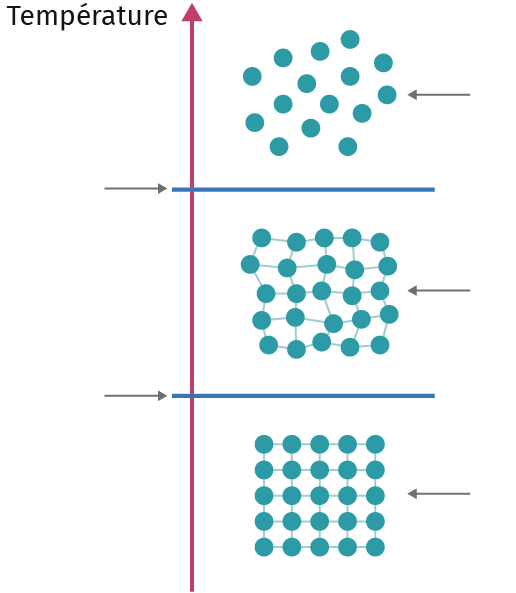
\includegraphics[width=0.6\linewidth]{evaluations/changement_etat.png}
\end{center}

\exo{Un fil de cuivre est :}{0}
\vspace*{-0.3cm}
\begin{qcm}
  \item Un corps pur.
  \item Un mélange.
  \item Une solution.
\end{qcm}